\section{Experiments}\label{sec:exp}

\subsection{Protocol}\label{sec:exp:protocol}

\paragraph{Data and evaluation.}
In-domain training uses the fixed SDSD~\citep{sdsd} split:
$136$ training sequences, $16$ validation sequences, and $39$ test sequences.
Scene groups are kept together when defining validation; sequences identified
as leaking between training and test were removed before this round.
For transfer we treat SDSD, BVI-RLV~\citep{bvi_rlv}, and
LOL~\citep{lol_v1,lol_v2} as three domains.
BVI-RLV has $48/16/16$ train/validation/test clips from $24/8/8$ scenes.
The LOL domain pools LOL-v1, LOL-v2-real, and LOL-v2-synthetic, with
$215$ test images in total.
Leave-one-domain-out training samples each of the two source domains with
probability $1/2$; neither source arm sees the held-out domain.

Videos use the centre $16$ frames and a $256\times256$ centre crop.
Frames are paired by sorted index rather than filename.
LOL images are evaluated at full resolution, repeated to form the encoder's
clip input; the single image prediction is scored.
PSNR-Y is computed after uint8 rounding, using the evaluator's BT.601 luma
conversion. LPIPS uses AlexNet~\citep{lpips}.
Temporal diagnostics include LPIPS between adjacent frames (tLP), reported
as the absolute gap to the target clip's value after seed-averaging within
each arm. Such diagnostics remain sensitive to
motion and are not interchangeable with perceptual reconstruction quality.

\paragraph{Decision rule.}
The main in-domain comparison has three seeds; transfer and most interventions
have two. Differences are paired by sequence after averaging within each arm
over seeds. We use $10{,}000$ sequence-bootstrap samples for $95\%$ intervals.
A claimed effect must exclude zero and have the same sign in every seed.
These intervals describe test-sequence variation conditional on the trained
models; the sign check does not replace estimating uncertainty over a larger
population of training seeds.
Unless specified otherwise, $\Delta$ means intervention minus reference,
so higher PSNR and lower LPIPS are better.

\subsection{The prior helps in domain}\label{sec:exp:control}

\begin{table}[t]
\centering\small
\setlength{\tabcolsep}{5pt}
\begin{tabular}{lcc}
\toprule
Conditioning / model & PSNR-Y $\uparrow$ & LPIPS $\downarrow$\\
\midrule
Zero tokens & \R{indomain@abs@none} & \R{indomain@abs@none@lpips}\\
Pretrained tokens & \R{indomain@abs@prior} & \R{indomain@abs@prior@lpips}\\
\midrule
Retinexformer, retrained & \R{rf@abs@psnr} & \R{rf@abs@lpips}\\
\bottomrule
\end{tabular}
\caption{SDSD test, $n=\R{indomain@n}$. Seer-v2 arms share architecture,
from-scratch recipe and the three nominal seeds. They do not share initial
pixel weights or training random draws (App.~\ref{app:stages}).
Retinexformer uses the same training split but its own architecture and
training schedule.}
\label{tab:control}
\end{table}

Pretrained conditioning improves the matched zero-token arm by
$\R{indomain@psnr}$\,dB
($\R{indomain@psnr@ci}$) and $\R{indomain@lpips}$ LPIPS
($\R{indomain@lpips@ci}$).
All three seeds agree in sign on both metrics.
The PSNR effect varies substantially across seeds, so its mean is evidence of
benefit under this protocol rather than a promise of a fixed improvement on
every run.
Because both arms start from scratch, this comparison avoids inheriting a
branch already adapted to the pretrained tokens.
The matched comparison alone does not separate the value of pretraining from
every possible alternative feature source.
The archived random control instantiated a different random encoder at
evaluation. Reusing the training seed instead yields
$\R{audit@random@psnr@b}$\,dB and
$\R{audit@random@lpips@b}$ LPIPS for that seed-zero checkpoint.
Against the corresponding pretrained seed, the differences are
$\R{audit@random@psnr}$\,dB ($\R{audit@random@psnr@ci}$) and
$\R{audit@random@lpips}$ LPIPS ($\R{audit@random@lpips@ci}$).
Only LPIPS resolves a benefit. This is a single trained random-control seed,
so its sequence interval cannot establish consistency over training seeds.

\paragraph{Comparison with a retrained restorer.}
Retinexformer~\citep{retinexformer} is retrained for $160{,}000$ steps on the
same SDSD training split.
Seer-v2's mean PSNR margin is $\R{vsrf@psnr}$\,dB
($\R{vsrf@psnr@ci}$), but its median is
$\R{vsrf@median}$\,dB and it wins only
$\R{vsrf@won}/\R{vsrf@n}$ sequences.
Its LPIPS difference is $\R{vsrf@lpips}$
($\R{vsrf@lpips@ci}$).
Neither interval excludes zero. The uneven sequence-level margin and different
model sizes preclude a claim of uniform superiority.
Our split and evaluation crop also differ from published benchmark tables,
so those absolute scores are not directly comparable.

\begin{figure*}[t]
\centering
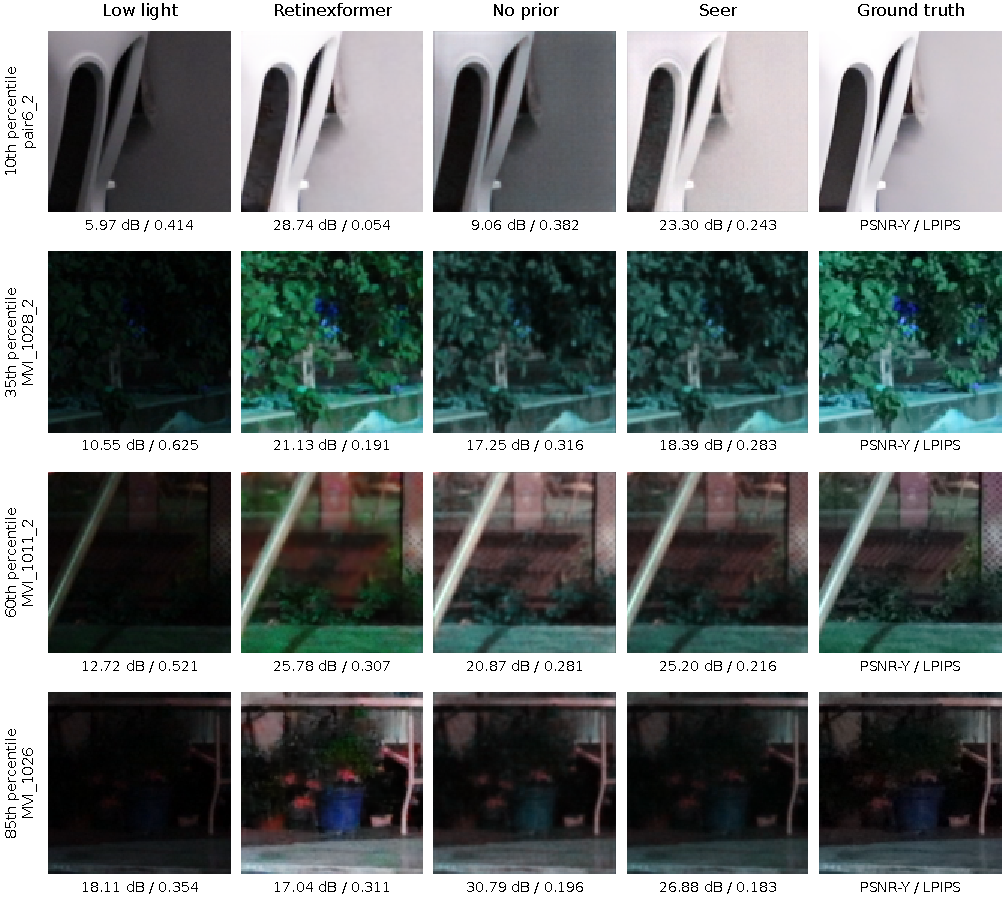
\includegraphics[width=\textwidth]{figures/fig_qualitative_cvpr.pdf}
\caption{Qualitative comparison, with columns showing input, retrained
Retinexformer, zero-token Seer-v2, pretrained Seer-v2, and ground truth.
Sequences are selected at four fixed quantiles of the sequence-level
PSNR-Y margin between the three-seed pretrained average and Retinexformer.
Displayed panel metrics score one middle frame, whereas the tables score
the full evaluation clip. Panels use pretrained and zero-token seed zero;
checkpoint, source and image hashes accompany the released figure.}
\label{fig:qualitative}
\end{figure*}

\subsection{The prior transfers under held-out-domain training}
\label{sec:exp:xdomain}

\begin{table*}[t]
\centering\small
\setlength{\tabcolsep}{8pt}
\begin{tabular}{lcll}
\toprule
Held out & $n$ & $\Delta$ PSNR-Y [95\% CI] & $\Delta$ LPIPS [95\% CI]\\
\midrule
SDSD & \R{xdom@sdsd@n} &
\R{xdom@sdsd@psnr}\ \R{xdom@sdsd@psnr@ci} &
\R{xdom@sdsd@lpips}\ \R{xdom@sdsd@lpips@ci}\\
BVI-RLV & \R{xdom@bvi@n} &
\R{xdom@bvi@psnr}\ \R{xdom@bvi@psnr@ci} &
\R{xdom@bvi@lpips}\ \R{xdom@bvi@lpips@ci}\\
LOL & \R{xdom@lol@n} &
\R{xdom@lol@psnr}\ \R{xdom@lol@psnr@ci} &
\R{xdom@lol@lpips}\ \R{xdom@lol@lpips@ci}\\
\bottomrule
\end{tabular}
\caption{Leave-one-domain-out transfer: pretrained minus zero-token
conditioning, two seeds per arm. A domain passes the registered rule when one
metric improves significantly, every seed agrees on that metric, and the other
metric has no significant degradation. SDSD and BVI-RLV pass on LPIPS; LOL
passes on PSNR-Y.}
\label{tab:xdomain}
\end{table*}

The registered transfer criterion requires improvement on at least one metric
in at least two held-out domains, without significant degradation of the other
metric. All three domains satisfy it (Table~\ref{tab:xdomain}).
The metric that improves differs: perceptual distance on SDSD and BVI-RLV,
and luminance fidelity on LOL.
This supports transfer of useful conditioning under the specified source
mixtures. It does not establish simultaneous improvement on every metric or
universal transfer to arbitrary sensors.
LOL is an image-domain test, so its improvement supplies no evidence of
temporal transfer.

\subsection{What a converged branch tolerates}\label{sec:exp:sufficiency}

\begin{table}[t]
\centering\small
\setlength{\tabcolsep}{3pt}
\begin{tabular}{lcl}
\toprule
Inference intervention & Seeds & $\Delta$ PSNR-Y [95\% CI]\\
\midrule
Per-clip centred rank 4 & \R{suff@seeds} &
\makecell[l]{\R{suff@rank4@d}\\\R{suff@rank4@ci}}\\
Spatial mean & \R{suff@seeds} &
\makecell[l]{\R{suff@spatial@d}\\\R{suff@spatial@ci}}\\
Temporal mean & \R{suff@seeds} &
\makecell[l]{\R{suff@temporal@d}\\\R{suff@temporal@ci}}\\
\midrule
Fixed rank 4 & \R{gsuff@seeds} &
\makecell[l]{\R{gsuff@global4}\\\R{gsuff@global4@ci}}\\
Fixed rank 16 & \R{gsuff@seeds} &
\makecell[l]{\R{gsuff@global16}\\\R{gsuff@global16@ci}}\\
Fixed rank 64 & \R{gsuff@seeds} &
\makecell[l]{\R{gsuff@global64}\\\R{gsuff@global64@ci}}\\
\bottomrule
\end{tabular}
\caption{Inference-only interventions on full-token-trained checkpoints,
paired with their identity controls on the same $39$ SDSD clips.
Per-clip projection retains the full clip mean; fixed projection uses the
training-set mean and basis. The two blocks have different seed counts.}
\label{tab:sufficiency}
\end{table}

Keeping four principal directions of each clip's centred tokens improves
PSNR-Y by $\R{suff@rank4@d}$\,dB
($\R{suff@rank4@ci}$), with all three seeds agreeing.
The corresponding $1024$-dimensional mean and the basis itself remain
clip-dependent. This is evidence that much of the within-clip token variation
can be removed after training; it is not a four-dimensional representation of
the whole clip.

Spatial or temporal averaging does not produce a significant PSNR change.
Their intervals are broad: the data still admit losses of roughly
$\R{suff@spatial}$\,dB and $\R{suff@temporal}$\,dB, respectively.
Absence of a detected degradation is therefore weaker than equivalence or
proof that the original field carries no useful spatial or temporal detail.

Fixed rank-4 and rank-16 replacements significantly degrade PSNR; fixed
rank-64 does not.
The contrast establishes that this fixed low-rank replacement is less
compatible with the learned branch than the per-clip replacement.
Because Eqs.~\eqref{eq:cliprank} and~\eqref{eq:globalrank} differ in both mean
and basis, that contrast cannot assign the gap solely to basis adaptivity.
Nor does it establish that the frozen encoder is impossible to replace.

\paragraph{Separating mean and basis on validation.}
An exploratory follow-up crosses both factors on all
$\R{meanval@n}$ SDSD validation sequences
($\R{meanval@scenes}$ scenes, $\R{meanval@seeds}$ existing seeds;
App.~\ref{app:meanbasis}).
Holding the clip mean fixed, adaptive rather than fixed rank-four directions
change PSNR-Y by $\R{meanval@clipvsfixed@psnr}$\,dB, with unadjusted
scene-bootstrap interval $\R{meanval@clipvsfixed@psnr@sceneci}$ and
positive effects in both seeds. Holding either basis fixed also favours the
clip mean over the training mean. This implicates both factors on validation;
it does not establish a training bottleneck or a cheaper encoder.
Rank-four projection versus identity remains inconclusive on this split.

Training-time projection addresses a different question.
The archived fixed-rank training evaluation did not restore its input
projection. Corrected evaluation applies the saved training-set mean and
rank-$64$ basis at inference as well.
Against full-token-trained seeds zero and one, its PSNR difference is
$\R{audit@grank64@psnr}$\,dB
($\R{audit@grank64@psnr@ci}$), and its LPIPS difference is
$\R{audit@grank64@lpips}$ ($\R{audit@grank64@lpips@ci}$).
The per-seed PSNR differences have opposite signs.
Neither interval resolves a difference, so the earlier significant
training-time penalty is withdrawn. These intervals also do not establish
equivalence or a faster model: the projection still follows the full encoder.

\subsection{Injection changes have mixed outcomes}
\label{sec:exp:ablation}

Restoring the saved hybrid key/value configuration also changes its archived
evaluation. Against the corresponding per-tubelet seeds zero and one,
hybrid keys change PSNR-Y by $\R{audit@hybrid@psnr}$\,dB
($\R{audit@hybrid@psnr@ci}$) and LPIPS by
$\R{audit@hybrid@lpips}$ ($\R{audit@hybrid@lpips@ci}$).
LPIPS improves in both seeds; PSNR remains unresolved.
This supports a modest perceptual benefit for this tested key/value variant.

Spatial grounding adds positional correspondence between pixel queries and
token keys. Over two seeds, its PSNR difference is
$\R{inj@spatial@psnr}$\,dB
($\R{inj@spatial@psnr@ci}$), and its LPIPS difference is
$\R{inj@spatial@lpips}$ ($\R{inj@spatial@lpips@ci}$).
Neither metric resolves an improvement at convergence.

Exposure decoupling adds a predicted global gain and a supervised exposure
objective. In its two-seed comparison, PSNR changes by
$\R{inj@edc@psnr}$\,dB ($\R{inj@edc@psnr@ci}$), while LPIPS changes by
$\R{inj@edc@lpips}$ ($\R{inj@edc@lpips@ci}$), both worse.
The spatial and exposure interventions do not justify their added structure
under this protocol. A corrected all-depth comparison is limited to one
variant seed with different training hardware (App.~\ref{app:pending});
deepest-only taps and learned gates still await verified evaluation.

\subsection{A temporal objective engages a different target}
\label{sec:exp:temporal}

The encoder is sensitive to temporal structure on this data.
The archived eight-clip probe detects a substantial block-23 token change
after shuffling under its relative token-distance measure.
This is a measurement of the encoder, separate from the restorer.

The relative temporal loss reduces the latent magnitude ratio to
$\R{h17@tdrel@mag}$ and leaves directional agreement at
$\R{h17@tdrel@cos}$.
Its LPIPS and tLP-gap changes are
$\R{h17@tdrel@lpips}$ ($\R{h17@tdrel@lpips@ci}$) and
$\R{h17@tdrel@tlp}$ ($\R{h17@tdrel@tlp@ci}$), respectively:
the loss rewards a smaller latent variation without improving the measured
reconstruction.

The cosine form restores the magnitude ratio to $\R{h17@tdcos@mag}$ and
reaches directional agreement $\R{h17@tdcos@cos}$.
Nevertheless LPIPS worsens by $\R{h17@tdcos@lpips}$
($\R{h17@tdcos@lpips@ci}$) and the tLP gap worsens by
$\R{h17@tdcos@tlp}$ ($\R{h17@tdcos@tlp@ci}$).
PSNR is unresolved:
$\R{h17@tdcos@psnr}$\,dB ($\R{h17@tdcos@psnr@ci}$).
The archived order probe for this model changes aggregate PSNR by only
$\R{ordersens}$\,dB after shuffling.
These observations distinguish matching latent temporal differences from
improving the pixel-space result; the former does not guarantee the latter.

\subsection{Why training budget belongs in the conclusion}
\label{sec:exp:budget}

The initial short-budget round and the converged round lead to different
decisions about the conditioning benefit, transfer, and temporal interventions.
Consequently, all effect estimates used above come from the fixed
$20{,}000$-step schedule, and early results are kept as exploratory records.
A conclusion about a small architectural effect requires that the reference
and intervention have both been trained long enough to make that comparison
meaningful. This is a protocol requirement demonstrated by this study, rather
than a proposed universal iteration count.
